\subsection{DYNKIN GRAPHS}

By abuse of language, we shall call a normed graph a pair \((\Gamma, f)\) having the following properties:

\begin{enumerate}
\def\labelenumi{\arabic{enumi})}
\item
  \(\Gamma\) is a graph (called the underlying graph of \((\Gamma, f)\) ).
\item
  If E denotes the set of pairs \((i,j)\) such that \(\{i,j\}\) is an edge of \(\Gamma\) . f is a map from E to R such that \(f(i,j)f(j,i)=1\) for all \((i,j)\in\mathbf{E}\) .
\end{enumerate}

There is an obvious notion of isomorphism of normed graphs.

Let R be a reduced root system in a real vector space V. We are going to associate to it a normed graph \((X, f)\) , called the Dynkin graph of R. The vertices of X will be the elements of the set I of orbits of W(R) in the union of the sets \(\{B\} \times B\) (where B is the set of bases of R). If \(N = (n_{ij})_{i,j \in I}\) (resp. \(M = (m_{ij})_{i,j \in I}\) ) is the canonical Cartan matrix (resp. the Coxeter matrix) of R ( \(\S\) 1, no. 5, Remark 7), two vertices i and j of X are linked if and only if \(n_{ij} \neq 0\) and we then put

\[
f (i, j) = \frac {n _ {i j}}{n _ {j i}}.
\]

Since \(n_{ij} = 0\) implies \(n_{ji} = 0\) , this defines a normed graph (X. f).

Let \((x|y)\) be a scalar product on V. invariant under W(R), and let \(B = (\alpha_i)_{i \in I}\) be a basis of R. indexed canonically. Formulas (7) and (9) of § 1. no. 1 show that vertices i and j of the graph X are linked if and only if

\[
(\alpha_ {i} | \alpha_ {j}) \neq 0
\]

and that

\[
f (i, j) = \frac {\left(\alpha_ {j} \mid \alpha_ {i}\right)}{\left(\alpha_ {j} \mid \alpha_ {j}\right)}.
\]

In view of the results of § 1, Nos. 3 and 5, the only possibilities are the following, up to interchanging \(i\) and \(j\) :

\begin{enumerate}
\def\labelenumi{\arabic{enumi})}
\item
  \(i\) and \(j\) are not linked; \(n_{ij} = n_{ji} = 0\) ; \(m_{ij} = 2\) ;
\item
  \(f(i,j) = f(j,i) = 1; n_{ij} = n_{ji} = -1; m_{ij} = 3;\)
\item
  \(f(i,j) = 2\) , \(f(j,i) = 1/2\) ; \(n_{ij} = -2\) . \(n_{ji} = -1\) ; \(m_{ij} = 4\) ;
\end{enumerate}

\[
f (i, j) = 3, f (j, i) = 1 / 3: n _ {i j} = - 3, n _ {j i} = - 1; m _ {i j} = 6.
\]

We see from this that the Dynkin graph R determines the Cartan matrix and the Coxeter matrix of R, and hence determines R up to isomorphism. More precisely, the Cor. of Prop. 15 of § 1, no. 5 implies the following result:

PROPOSITION 1. Let \(R_{1}\) and \(R_{2}\) be two reduced root systems in vector spaces \(V_{1}\) and \(V_{2}\) . Let \(B_{1} = (\alpha_{i})_{i \in I_{1}}\) and \(B_{2} = (\alpha_{i})_{i \in I_{2}}\) be bases of \(R_{1}\) and \(R_{2}\) , indexed canonically. Let \(\lambda\) be an isomorphism from the Dynkin graph of \(R_{1}\) to the Dynkin graph of \(R_{2}\) . Then, there exists a unique isomorphism from \(V_{1}\) to \(V_{2}\) transforming \(R_{1}\) into \(R_{2}\) and \(\alpha_{i}\) into \(\alpha_{\lambda(i)}\) for all \(i \in I_{1}\) .

It is clear that an automorphism of R defines an automorphism of the Dynkin graph of R, and hence a homomorphism \(\varphi\) from the group A(R) to the group of automorphisms of the Dynkin graph of R.

COROLLARY. The homomorphism \(\varphi\) defines by passage to the quotient an isomorphism from the group A(R)/W(R) to the group of automorphisms of the Dynkin graph of R.

Clearly, \(\varphi(g) = \operatorname{Id}\) for all \(g \in W(R)\) . On the other hand, Prop. 1 shows that there exists an isomorphism \(\psi\) from the group of isomorphisms of the Dynkin graph of \(R\) to the subgroup \(E\) of elements of \(A(R)\) leaving fixed a given basis \(B\) of \(R\) , such that \(\varphi \circ \psi = \operatorname{Id}\) . Since \(A(R)\) is the semi-direct product of \(E\) and \(W(R)\) (§ 1, no. 5, Prop. 16), the corollary follows.

In practice, the Dynkin graph \((X, f)\) is represented by a diagram composed of nodes and bonds in the following way. The nodes correspond to the vertices of X; two nodes corresponding to two distinct vertices i and j are joined by 0, 1, 2 or 3 bonds in cases 1), 2), 3) and 4) above (up to interchanging i and j). Moreover, in cases 3) and 4), that is when \(f(i, j) > 1\) , or when the roots \(\alpha_{1}\) and \(\alpha_{j}\) are not orthogonal and not of the same length, an inequality sign \textgreater{} is placed on the double or triple bond joining the nodes corresponding to i and j oriented towards the node corresponding to j (that is, the shortest root):

\[
\underset {i} {\longrightarrow} \underset {j} {\longrightarrow} \quad (\text { for   } f (i, j) = 2), \quad \underset {i} {\longrightarrow} \underset {j} {\longrightarrow} \quad (\text { for   } f (i, j) = 3).
\]

It is clear that the Dynkin graph \((X, f)\) can be recovered from this diagram.

We remark that the diagram associated to the Coxeter graph of W(R) can be obtained from that associated to the Dynkin graph of R by keeping the nodes and the single bonds and replacing the double (resp. triple) bonds by a bond surmounted by the number 4 (resp. 6). Conversely, given the Coxeter graph of W(R), the diagram associated to the Dynkin graph of R can be recovered using the inverse of this procedure, except for the inequality signs on the double or triple bonds. Th. 1 thus gives immediately the list of possible Dynkin graphs. More precisely:

THEOREM 3. If R is an irreducible reduced root system, its Dynkin graph is isomorphic to one of the graphs represented by the following diagrams:

\pandocbounded{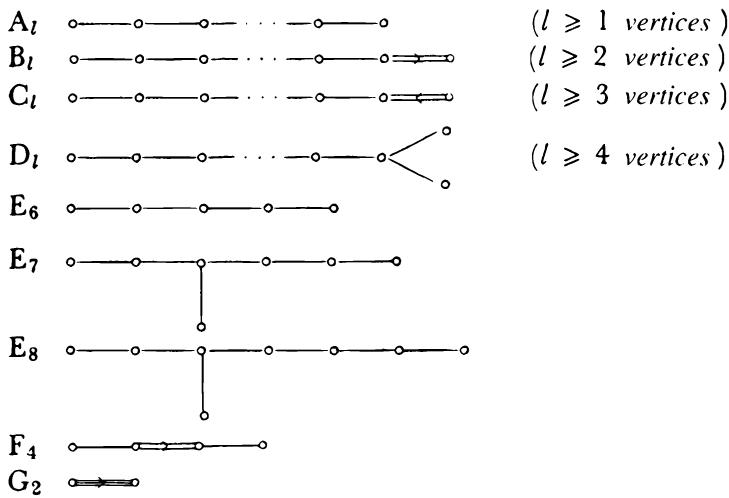
\includegraphics[keepaspectratio]{images/part002_c37a5a77.jpg}}

No two of these graphs are isomorphic and there are irreducible reduced root systems having each of them as their Dynkin graph (up to isomorphism).

The first assertion follows immediately from Th. 1, in view of the preceding remarks, the fact that the Coxeter groups of the graphs \(H_{3}\) , \(H_{4}\) and \(I_{2}(p)\) (for p = 5 and \(p \geqslant 7\) ) are not crystallographic, and the fact that the two possible inequalities for the double (resp. triple) bond of the Dynkin graph associated to the Coxeter graph \(F_{4}\) (resp. \(G_{2}\) ) give isomorphic Dynkin graphs. The second assertion is clear and the third will follow from the explicit construction of an irreducible reduced root system for each type, a construction that will be carried out in Nos. 5 to 13.

Remarks. 1) The graph \(A_{1}\) reduces to a single node; we denote it also by \(B_{1}\) or \(C_{1}\) . The graph \(B_{2}\) is also denoted by \(C_{2}\) . The graph \(A_{3}\) is also denoted by \(D_{3}\) . Finally, \(D_{2}\) denotes the graph consisting of two unconnected nodes. (These conventions are derived from the properties of the corresponding root systems, cf.~nos. 5 to 8.)

\begin{enumerate}
\def\labelenumi{\arabic{enumi})}
\setcounter{enumi}{1}
\tightlist
\item
  If \((X, f)\) is the Dynkin graph of a reduced root system R. the Dynkin graph of the inverse system can be identified with \((X, f^{-1})\) . In other words, the diagram associated to the Dynkin graph of \(R^{\prime}\) can be obtained from that associated to the Dynkin graph of R by reversing the inequality signs. If R is irreducible, we see that R is isomorphic to \(R^{\prime}\) unless R is of type \(B_{l}\) or \(C_{l}\) , in which case \(R^{\prime}\) is of type \(C_{l}\) or \(B_{l}\) .
\end{enumerate}

